%%
%%
%%      SECTION: SENSITIVITY
%%

%% \begin{figure}[htpb]
%% \begin{center}
%% %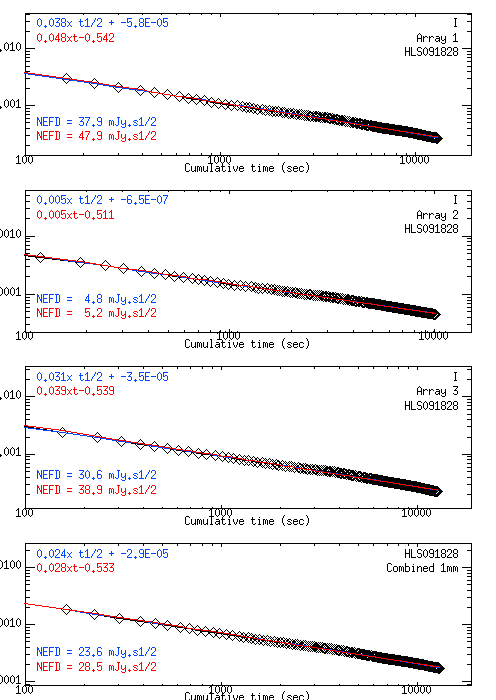
\includegraphics[clip, angle=0, scale =
%% %  0.5]{Figures/NEFD_HLS091828_20170226s415_FXDC0C1_GaussPhot.png}
%% %\includegraphics[clip, angle=0, scale = 0.5]{Figures/nefd_mpfit_HLS091828.eps}
%% \includegraphics[clip, angle=0, scale = 0.4]{Figures/HLS_fit.eps}
%% \includegraphics[clip, angle=0, scale = 0.4]{Figures/HLS_residuals.eps}
%% \caption{Sensitivity on \hls\ vs time of integration. Two power laws are fit:
%%   one with fixed slope $t^{1/2}$ that provides the estimate of the NEFD, one
%%   with a free slope $t^\beta$ to monitor the departure of noise integration from
%%   the canonical $t^{1/2}$. These data come from the integration on \hls\ during
%%   Run9. The difference between the 1 and 2~mm integration time comes from the
%%   density of KIDs in the FOV.}
%% \label{fig:nefd_vs_t}
%% \end{center}
%% \end{figure}

%% {\bf The specs/goals ``NEFD on X \% of pixels'' should be understood as : we have
%% XX\% valid pixels, and with these pixels, we have an NEFD of YY. We should not
%% discard some fraction of our pixels and estimate an NEFD on this subset.}\\

\section{Methodology {\color{blue} Nico}}

The MoU defines the NEFD:  \emph{The Noise Equivalent Flux Density (NEFD)
  is the $1\,\sigma$ sensitivity in one second of effective on-source telescope
  integration time after the absolute calibration has been performed (i.e. after
  beam efficiency and opacity corrections). It is appropriate for 2 mm of
  precipitable water vapor (pwv) content in the atmosphere and 60 degrees
  elevation source. It refers to the inverse variance of the noise on the flux
  measurement of a point-source, averaged over the valid receiver pixels}.

IRAM has its own time estimator that will compute the ``effective NEFD'',
provided we give the ``detector NEFD'' and a fraction of valid KIDs. We must be
careful not to mix both, which has been the case in several ways. We must not
mix the intuitive definition of the NEFD and that of the mapping speed as well :
in short, NIKA2's NEFD must be the same as NIKA's NEFD, but NIKA2's larger FOV
improves the mapping speed. All this was hidden in the definition of $\eta$ in
the previous version of this doc that I hope to clarify here.\\

\subsection{Estimating the time of integration}

To compute the instrumental NEFD (hereafter NEFD), we must compute the
integration time on the source. This time is the total time spent by detectors
measuring the source, \emph{not} by the matrix footprint. Let's be more
specific: if the source is in the focal plane, but on a place where no KID is
valid, the integration time is zero. There are 3 ways to estimate the time of
integration. We introduce them in the following 3 subsections and compare them
on Fig.~\ref{fig:time_comparison}.

\subsubsection{Time of integration from the density of samples}

Let's take a map of resolution $r$. The number of hits in the central pixel on
the source $N_h(r)$ leads to:

\begin{equation}
t_{int} = \frac{N_h(r)}{\nu}\frac{1}{N_{kids\,per\,pixel}}
\end{equation}

Suppose we stay fixed on the source (no movement at all) during a time $t_{obs}$, and $r$ is such that
there is only one KID staring at the source, then

\begin{equation}
t_{int} = \frac{1}{\nu}t_{obs}\times\nu = t_{obs}
\end{equation}

Suppose there are two kids per pixels, then the number of hits is twice as large
while $t_{obs}$ remains the same. In practice, this factor
$N_{kids\,per\,pixel}$ is difficult to estimate exactly because it depends on the
scanning strategy and the repartition of KIDs accross the FOV. In practice, we
are bound to compute averages and thus to estimate the average number of KIDs
per map pixel which is 

\begin{equation}
N^{avg}_{kids\,per\,pixel} = r^2/g^2
\end{equation}

where $g$ is the grid step of a matrix. Indeed, the total surface coverged by
$N_{kids}$ detectors is $S = N_{kids}g^2$ and there are $S/r^2$ map pixels in
this surface. So, the integration time on the source is finally

\begin{equation}
t_{int} = \frac{N_h(r)}{\nu}\frac{g^2}{r^2}\,.
\label{eq:t_int}
\end{equation}

Another justification of this formula is that $N_h(r)/r^2$ is the density of
samples in hits/arcsec$^2$ and $g^2$ is the inverse of the number of KIDs per
arcsec$^2$. For the combined 1mm, we must divide by 2 because both matrices
observe the same area at the same time:

\begin{equation}
t^{1mm}_{int} = \frac{1}{2}\frac{N_h(r)}{\nu}\frac{g^2}{r^2}\,.
\label{eq:t_int_1mm}
\end{equation}

So finally:

\begin{equation}
NEFD = \sigma \sqrt{t_{int}}
\label{eq:nefd_t_int}
\end{equation}

With this definition in hand, assuming we have only $N_{valid}$ kids in a focal
plane of $N_{full}$ KIDs in theory, we can, as a rule of thumb, estimate
the required time of integration required to reach a sensitivity
$\sigma_{target}$. Let's call $\eta = N_{valid}/N_{full}$ the fraction of valid
KIDs of the matrix. To reach the same number of hits per map pixels, with the
same scanning strategy, the total integration time must be $1/\eta$ time larger,
hence : 

\begin{equation}
t_{astronomer} = \left(\frac{NEFD}{\sigma_{target}}\right)^2\frac{1}{\eta}
\label{eq:t_astro}
\end{equation}

\subsubsection{Time of integration from the matrix footprint}

One can also think of the ``time spent on the source'', for a full matrix
(ie. all valid KIDs), as the time when the source is inside the circular
footprint of the matrix. During a scan, it's easy to count how much time the
source is at a distance from the FOV center that is larger than the FOV
radius. Let's call this time $t_{geom}$. However, because the map is produced
with only a fraction $\eta$ of valid KIDs, the effective integration time on the
source is $\eta$ times smaller than $t_{geom}$. Hence:

\begin{equation}
NEFD = \sigma \sqrt{t_{geom}\eta}
\label{eq:nefd_t_geom}
\end{equation}


\subsubsection{Time of integration from the flux estimator}

The NEFD is defined as the noise ``per beam'', the uncertainty on the estimation
of the flux of a point source. The estimation of a point source flux is given by
the fit of a gaussian profile, that in the case of white noise reduces to:

\begin{equation}
\hat{\phi} = \frac{1}{\sum_p g_p^2}\sum_p g_p m_p\,,
\label{eq:phi_def}
\end{equation}

and whose variance is

\begin{equation}
\sigma_\phi^2 = \left(\frac{1}{\sum_p g_p^2}\right)^2\sum_p g_p^2\sigma_p^2\,.
\label{eq:sigma_phi_def}
\end{equation}

In the case of white noise and considering the equivalent of the
uniform full matrix of the NEFD definition: $\sigma_p = \sigma/\sqrt{N_p}$,
where $\sigma$ is the standard deviation of 1 sample and $N_p$ is the number of
hits in pixel $p$. Accounting for the sampling frequency, it reads

\begin{eqnarray}
\sigma_\phi^2 &=& \frac{\sigma}{\nu}\left(\frac{1}{\sum_p g_p^2}\right)^2\sum_p \frac{g_p^2}{t_p}\,, \nonumber\\
&=&\frac{\sigma}{\nu}\frac{1}{t_{beam}}\,
\label{eq:sigma_phi_def_2}
\end{eqnarray}

where $t_{beam}$ is homogeneous to a time and is such that $\sigma_\phi$ goes
like $1/\sqrt{t_{beam}}$.\\


\begin{figure}
\begin{center}
\includegraphics[clip, angle=0, scale =0.8]{Figures/Pluto_time_of_integration.eps}
\caption[Time of integration]{Comparison between three estimators of the time of integration on the
  source during Pluto's observation (Run9). To a few percent, the 3 estimators
  give compatible estimations.}
\label{fig:time_comparison}
\end{center}
\end{figure}


%% Note: there is no way to be perfectly precise on the estimation of these
%% parameters, in all circumstances, on the edges of any matrix, for potential
%% areas covered by A1 and not A3 (or just less). Like in any case, we must live
%% with this, focus on the main area of each scan and forget about edge effects.

%\section{History and confusions}

%In the past few days, we have re-examined these definitions, and several
%mistakes were made:

%\begin{itemize}
%\item at some point, the {\tt nk\_map\_photometry.pro} that is supposed to give
%  the correct ``time'', rather than giving $t_{int}$ as defined in
%  Eq.~(\ref{eq:t_int}) was giving $\eta t_{int}$.
%\item When questioning this relation, we confused $t_{int}$ and $t_{obs} = t_{int}/\eta$. While
%  the dependence on the grid step and the map resolution was accounted for in
%  average, it was not the correct time to consider to compute the NEFD as defined in
%  the MoU (a.k.a detector NEFD, letting $\eta$ as another parameter in IRAM's
%  time estimator).
%\item In the end, the final NEFD we must give to IRAM are those that we
%  published but increased by a factor $1/\sqrt{\eta}$.
%\end{itemize}


\subsection{NEFD estimation methods}

To perform consistency and robustness test, we have developped three methods for the NEFD estimation. Namely, Methods 1 and 2 relie on deep integration on faint source: while Method 1 estimates the NEFD from a fit of the evolution of the flux density uncertainties with the integration time, Method 2 resorts to combining the scans in order to annulate the signal and obtain noise estimates. Detailed methodology and results are discussed in Sect.~\ref{NEFD_deep}. Method 3 consists in i) estimating an NEFD per point-source scan by evaluating the flux noise from map pixels far from the source and ii) studying the NEFD distribution as a function of the atmospheric attenuation to report the NEFD estimate for the appropiate observing conditions. Method 3 results are presented in Sect.~\ref{NEFD_pipeline}.     

